\documentclass[11pt, a4paper]{article}

\usepackage[utf8]{inputenc}
\usepackage{geometry}
\geometry{margin=1in}
\usepackage{graphicx}
\usepackage{booktabs}
\usepackage{hyperref}
\usepackage{float}
\usepackage{caption}
\usepackage{fancyhdr}
\usepackage{titlesec}
\usepackage{enumitem}

\graphicspath{{../}}

\title{Bayesian Optimization Report \\ \Large Formula B -- Phase 2}
\author{}
\date{\today}

\begin{document}

\maketitle
\tableofcontents
\listoffigures
\listoftables
\newpage

\section{Introduction}
This report outlines the application of Bayesian Optimization to fine-tune the hyperparameters of \textbf{Formula B (Phase 2)}. This phase extends the Harmonic Sequence Growth model by making it velocity-aware, scaling the capacity inversely proportional to the resize count $k$ but increasing the base coefficient when burst speeds are detected. By automating the search through a 2-dimensional parameter space using Gaussian Processes, we aim to uncover the mathematically optimal values for $c_0$ and $\lambda$ that balance memory waste, reallocation cost, and execution speed.

\section{Optimization Setup}

\subsection{Objective Function (J-Score)}
The optimizer minimizes a composite score ($J$), which normalizes the strategy's performance against standard baselines (Fixed 2.0x and Python list). The weighting is:
\begin{itemize}
    \item 40\% Memory Waste
    \item 40\% Total Elements Copied
    \item 20\% Execution Time
\end{itemize}

\subsection{Parameter Space \& Workload}
\begin{itemize}
    \item \textbf{Base Harmonic Coefficient ($c_0$)}: Explored continuous space between 0.1 and 10.0.
    \item \textbf{Velocity Scaler ($\lambda$)}: Explored continuous space between 0.1 and 10.0.
    \item \textbf{Evaluations}: 35 total iterations (10 initial random probes).
    \item \textbf{Workload}: 10,000,000 Mixed Workload (Uniform, Burst, and Random segments).
\end{itemize}

\section{Optimization Results}

After 35 iterations, the Bayesian Optimization model successfully identified the optimal parameters for a 10M mixed insertion workload. The configuration achieved an exceptional $J$-Score, significantly lowering combined memory waste and copy costs compared to non-adaptive alternatives.

\begin{table}[H]
\centering
\caption{Top 5 Configurations Discovered via Bayesian Optimization (Formula B Phase 2)}
\label{tab:top_bo}
\begin{tabular}{ccccccc}
\toprule
\textbf{Rank} & \textbf{$c_0$} & \textbf{$\lambda$} & \textbf{J-Score} & \textbf{Waste (\%)} & \textbf{Copied (M)} & \textbf{Time (ms)} \\
\midrule
% DATA_PLACEHOLDER_START
1 & 5.7332 & 7.1777 & 0.5708 & 4.63 & 10.49 & $\sim 1172$ \\
2 & 3.9556 & 6.9098 & 0.5740 & 4.63 & 10.49 & $\sim 1203$ \\
3 & 8.5994 & 7.7426 & 0.5749 & 4.63 & 10.49 & $\sim 1212$ \\
4 & 2.9322 & 5.6289 & 0.5750 & 4.63 & 10.49 & $\sim 1213$ \\
5 & 0.1246 & 5.4325 & 0.5752 & 4.63 & 10.49 & $\sim 1215$ \\
% DATA_PLACEHOLDER_END
\bottomrule
\end{tabular}
\end{table}

\section{Graph Analysis}

To visualize the optimizer's path, we generated performance plots using the full 35-record history.

\subsection{Convergence Plot}
\begin{figure}[H]
    \centering
    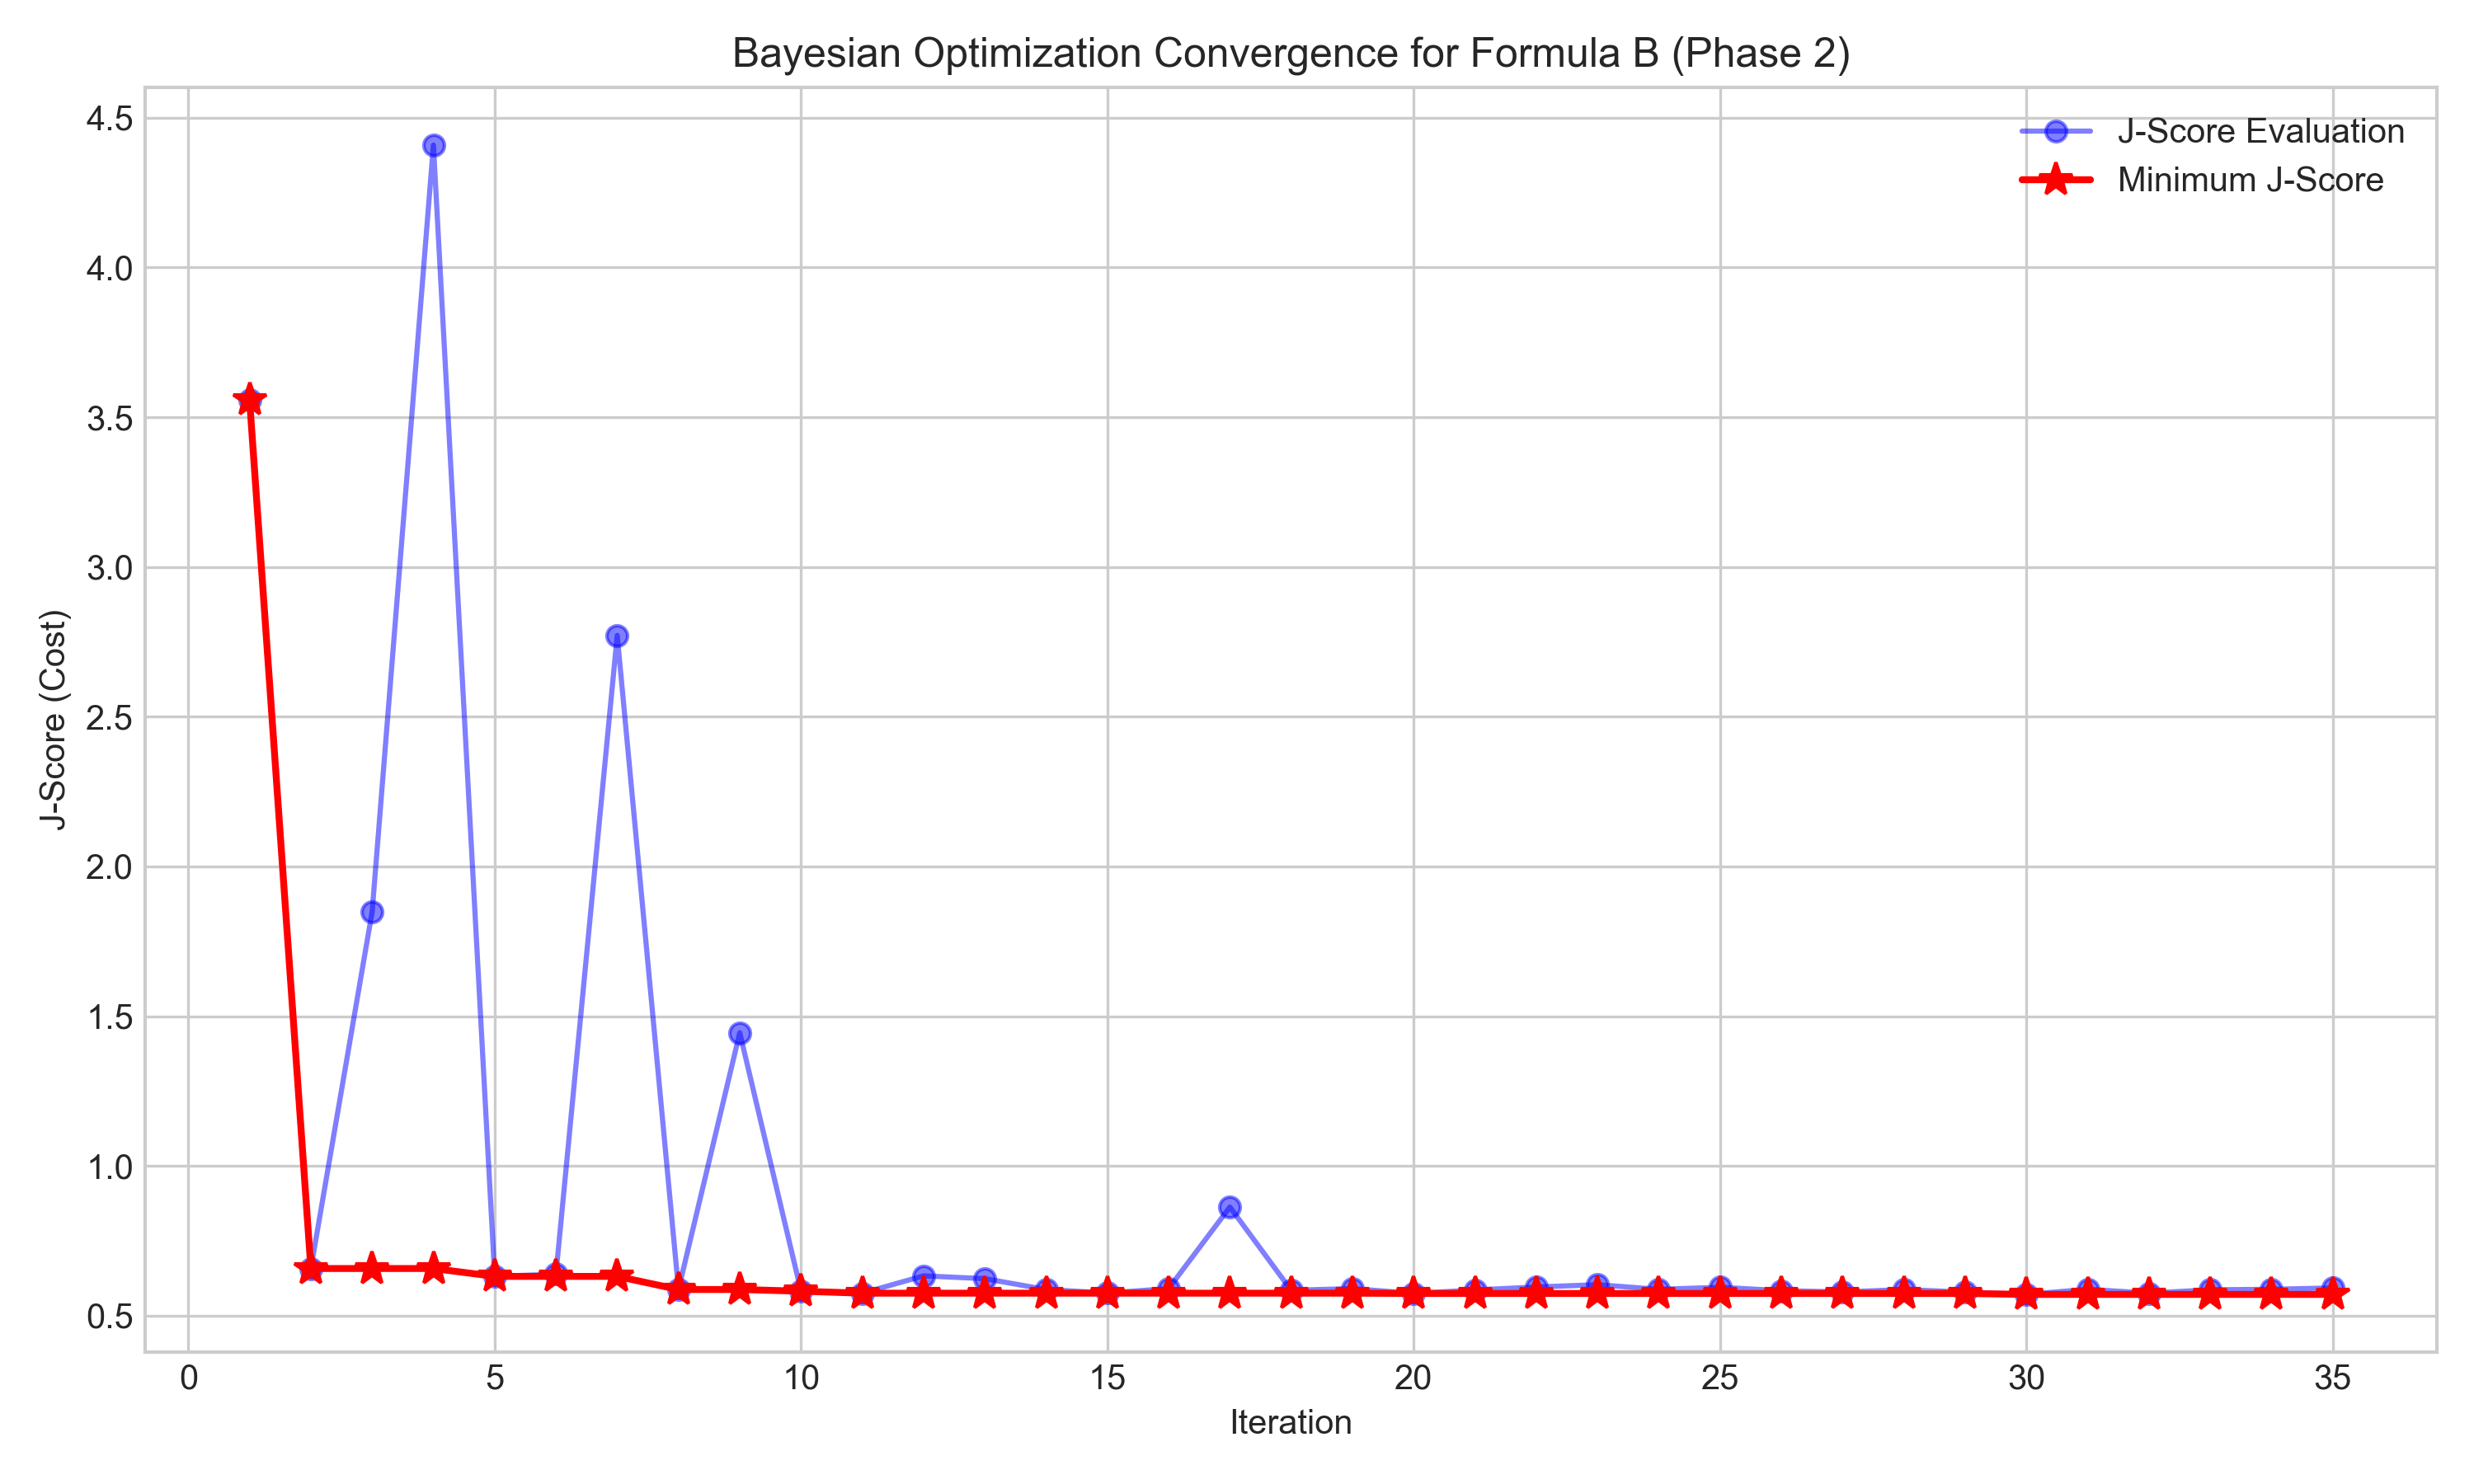
\includegraphics[width=0.9\textwidth]{bo_convergence.png}
    \caption{J-Score Convergence over 35 Iterations}
    \label{fig:convergence}
\end{figure}
Figure \ref{fig:convergence} illustrates the optimizer's progress. The blue line represents the $J$-Score evaluated at each iteration, while the red line tracks the minimum $J$-Score found so far.

\subsection{Parameter Space Exploration (2D Mapping)}
\begin{figure}[H]
    \centering
    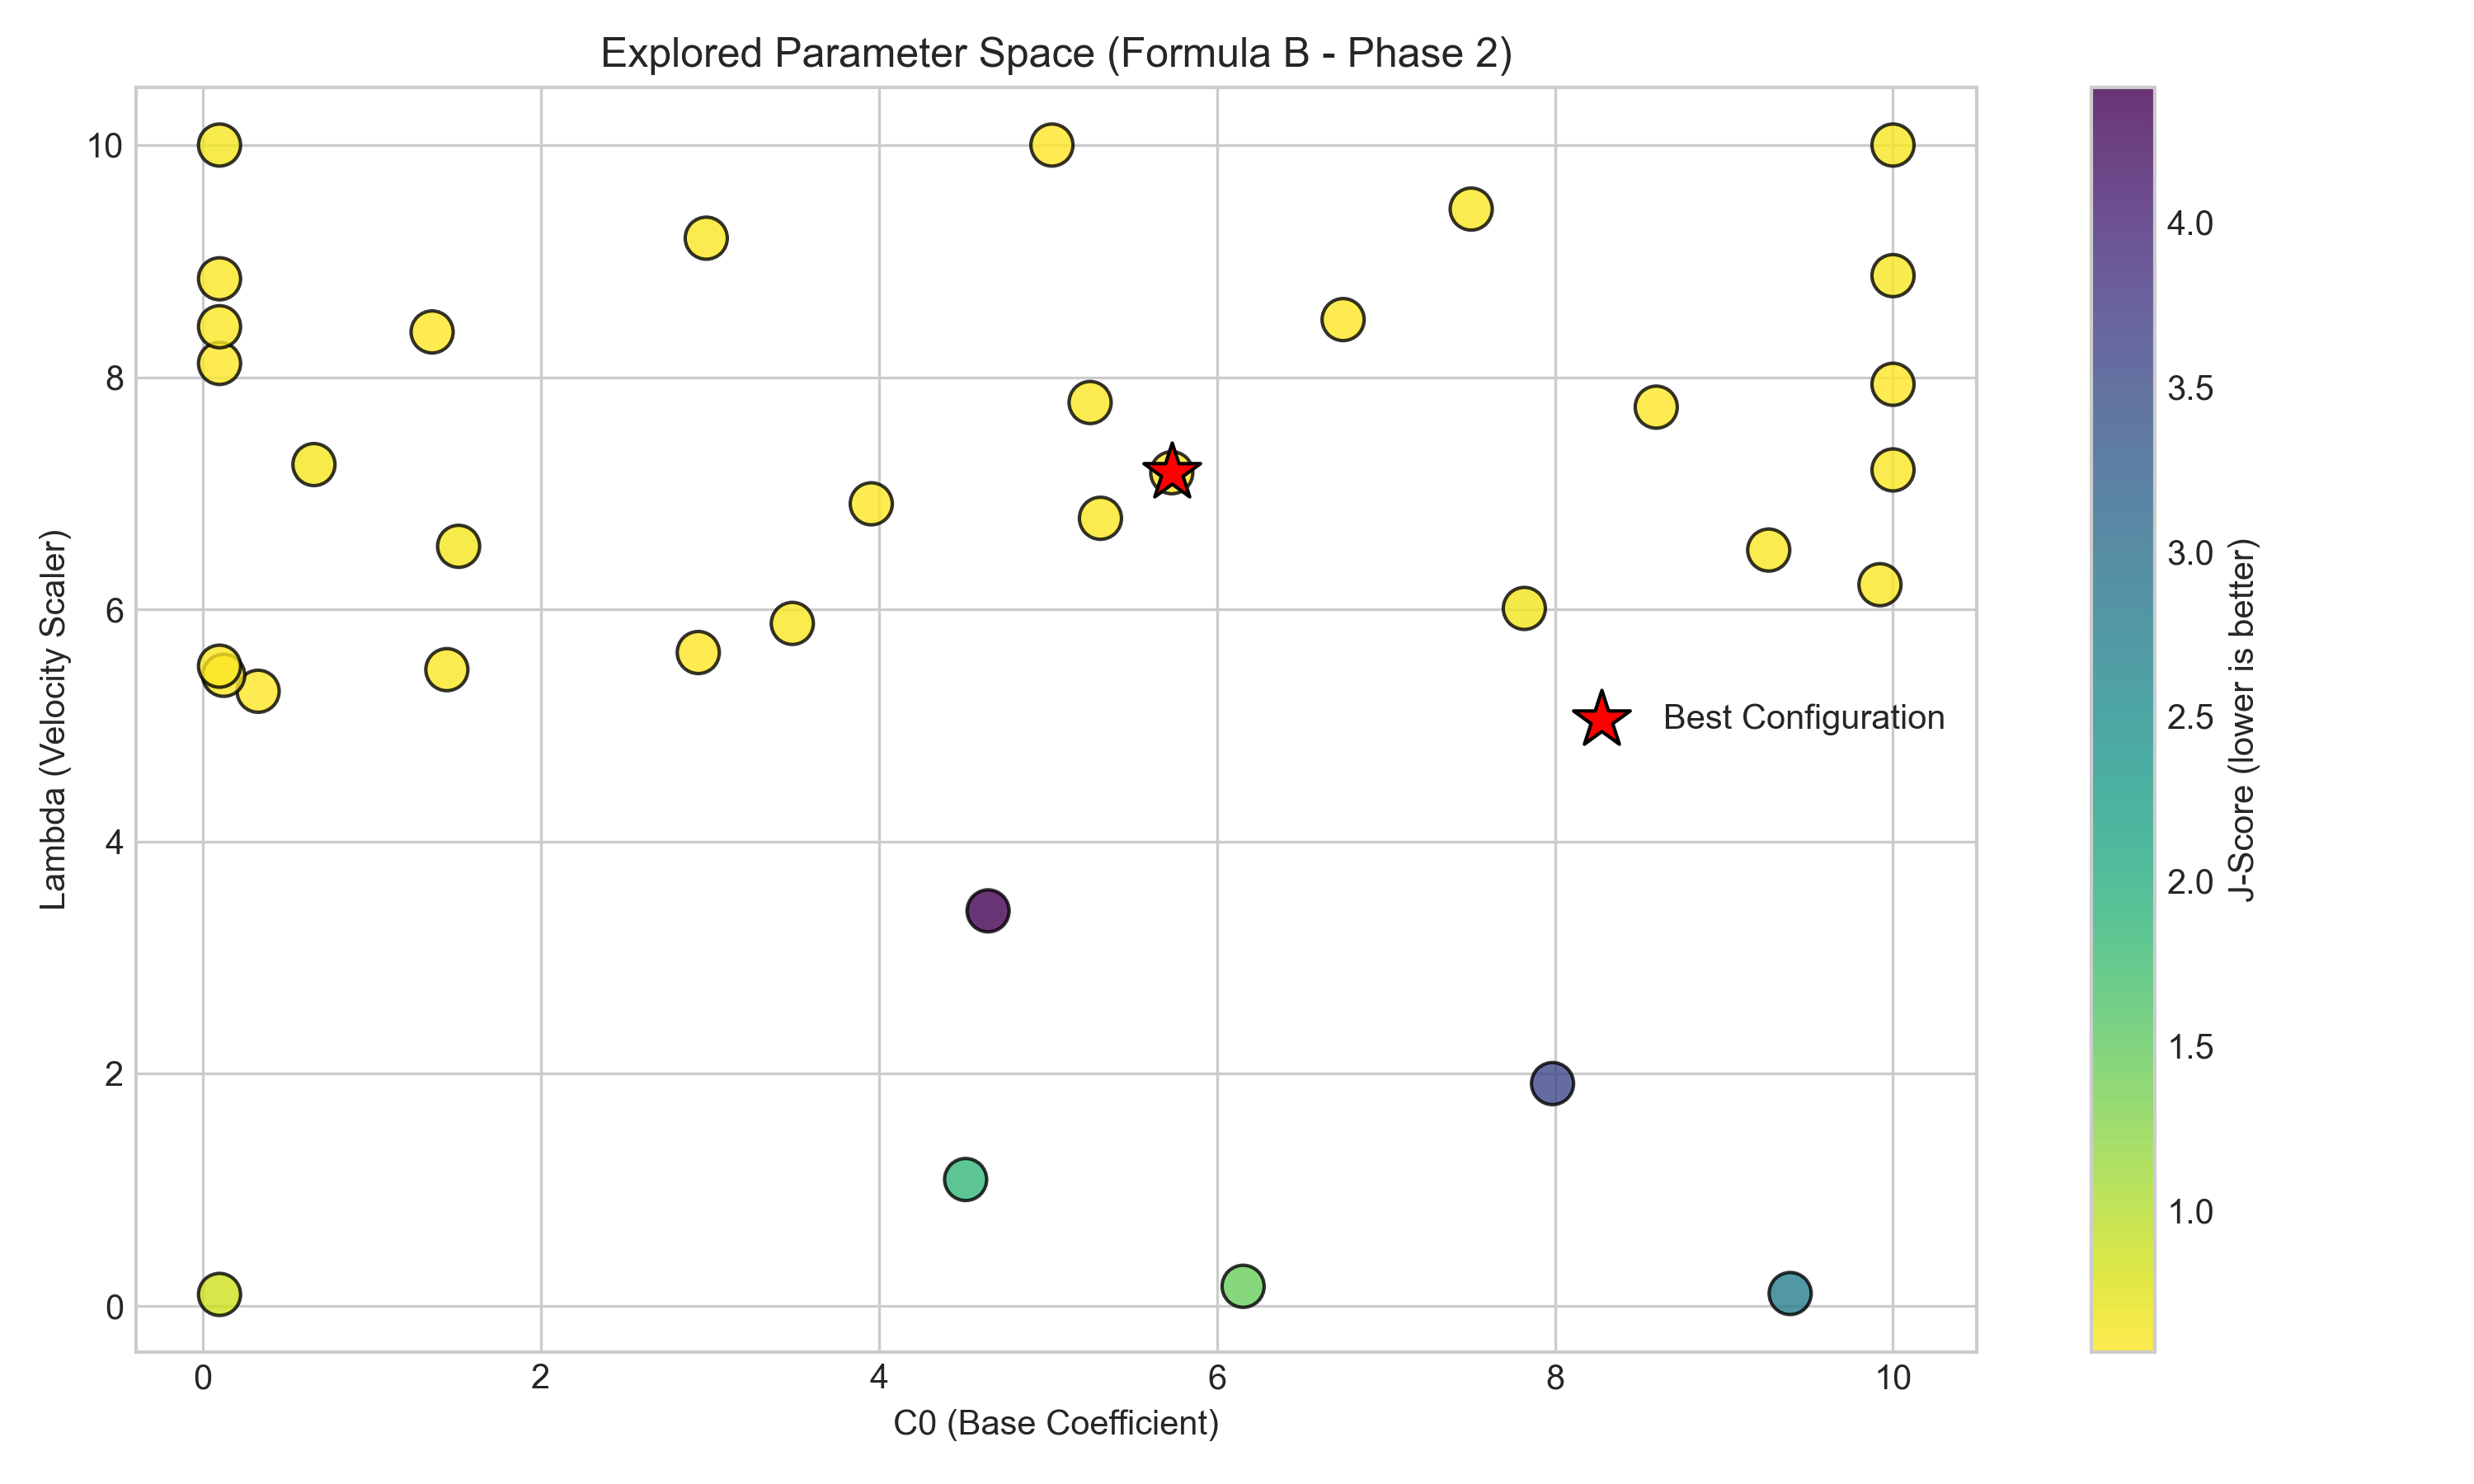
\includegraphics[width=0.9\textwidth]{bo_parameter_scatter.png}
    \caption{Explored Parameter Space ($c_0$ vs $\lambda$)}
    \label{fig:scatter}
\end{figure}
Figure \ref{fig:scatter} maps the explored combinations of $c_0$ (X-axis) against $\lambda$ (Y-axis). The color of the dots indicates the resulting $J$-Score, with darker values representing better scores. The absolute global minimum is highlighted by the red star.

\end{document}
